% --------------------------------------------------------------
\begin{frame}[fragile]
  \frametitle{Previous Work}
  \begin{itemize}
    \item Oak Ridge AHTR - unnecessary (Varma, Holcomb, et al.)
    \item Algebraic, 1-group LOFC neutronics analysis (Cisneros)
    \item Algebraic, 1-group RIA neutronics analysis (Greenspan, Fratoni)
    \item COMSOL TH response analysis (Huff, Scarlat)
  \end{itemize}

\end{frame}

% --------------------------------------------------------------
\begin{frame}[fragile]
  \frametitle{Unnecessary?}
  \begin{itemize}
    \item characterization of coolant, metal structure response
    \item characterization of startup strategy
    \item analysis of reactivity insertion behavior
    \item NRC required
  \end{itemize}
\end{frame}


% --------------------------------------------------------------
\begin{frame}[fragile]
  \frametitle{PB-FHR ATWS}

  \begin{columns}[t]
      \begin{column}{0.3\linewidth}
        \footnotesize{
        \begin{align}
        &T_{hot-shutdown} \approx \nonumber\\
        &\frac{
          \frac{\partial \rho}{\partial T_{f}}T_{f}+ 
                        \frac{\partial \rho}{\partial T_{c}}T_{c}}
                        {\frac{\partial \rho}{\partial T_{f}}+ 
                         \frac{\partial \rho}{\partial T_{c}}}\nonumber
        \end{align}
      }
      \end{column}
      \begin{column}{0.7\linewidth}
      \begin{figure}[h]
      \begin{center}
            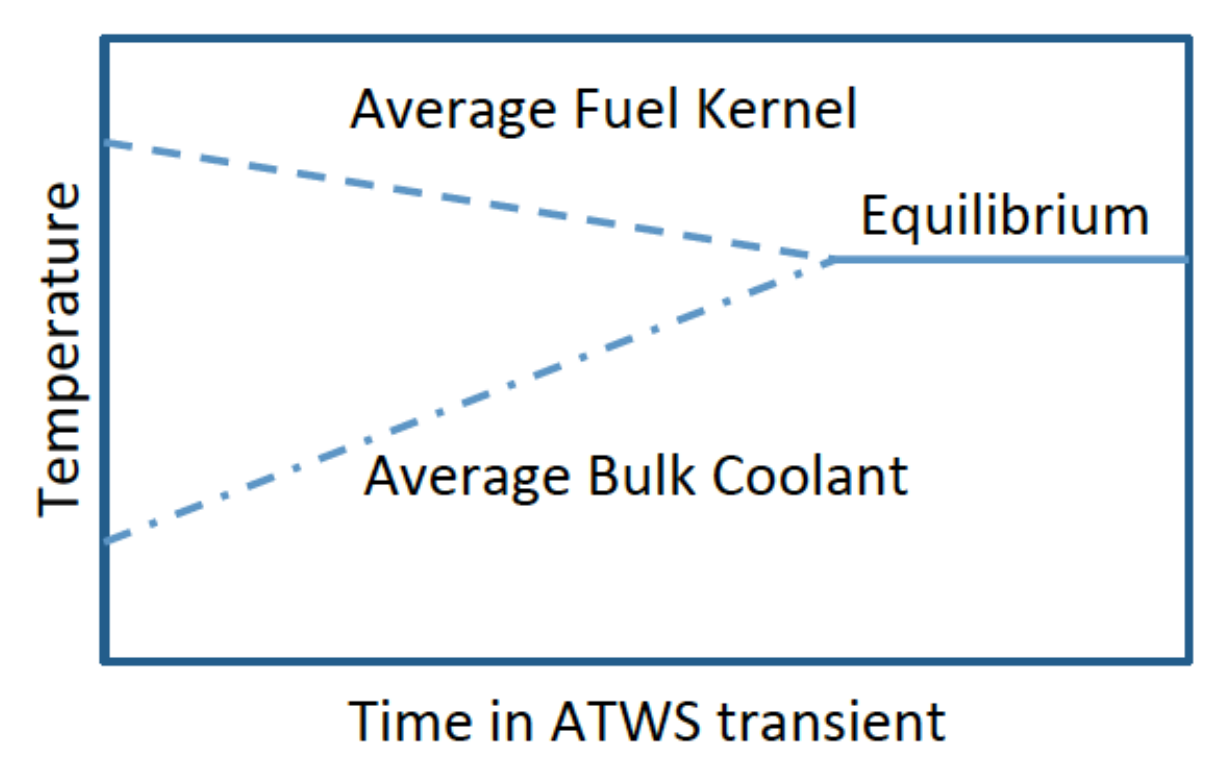
\includegraphics[width=0.7\textwidth]{./priorart/cisneros_atws.eps}
      \end{center}
        \caption{Temperature evolution of fuel kernel and coolant during a 
        hypothetical ATWS accident. Note the exact transition to equilibrium is 
        not known so this transition is represented with broken lines 
        [Cisneros, 2013].}
      \label{fig:cisneros_atws}
      \end{figure}
      \end{column}
    \end{columns}
\end{frame}

% --------------------------------------------------------------
\begin{frame}[fragile]
  \frametitle{PB-FHR ATWS}

      \begin{figure}[h]
      \begin{center}
            \includegraphics[width=0.6\textwidth]{./priorart/cisneros_coolant_atws.eps}
      \end{center}
        \caption{Temperature evolution of coolant during a 
        hypothetical ATWS accident, as afunciton of fuel design [Cisneros, 2013].}
      \label{fig:cisneros_atws}
      \end{figure}

\end{frame}

% --------------------------------------------------------------
\begin{frame}[fragile]
  \frametitle{PB-FHR RIA}
  Fuchs-Nordheim approximation idicates \$2 prompt reactivity insertion has max 
  fuel temperature of approximately $1200^{\circ}C$ [Greenspan, email]. This is 
  low enough for fuel survival.
\end{frame}


% --------------------------------------------------------------
\begin{frame}[fragile]
  \frametitle{Static COMSOL Model}

  \begin{figure}[htbp!]
    \begin{center}
      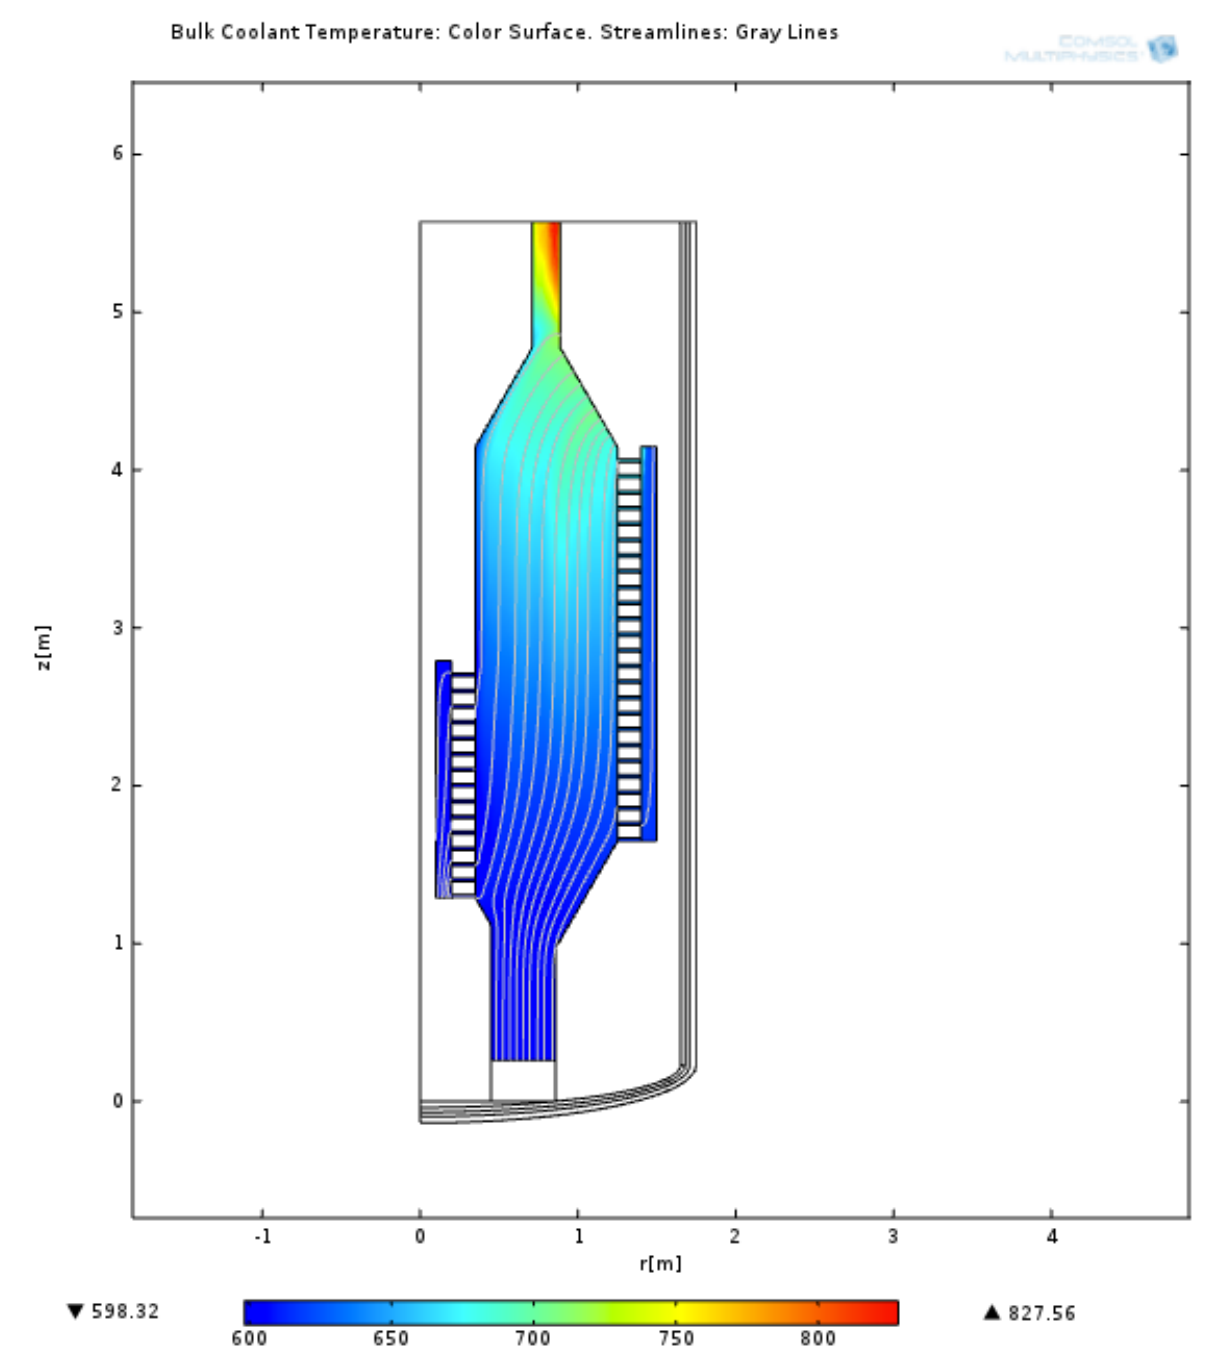
\includegraphics[height=0.8\textheight]{./priorart/coolant_temps_200_deg_rise.eps}
    \end{center}
    \caption{For 200 degree temperature rise design point across the core.}
    \label{fig:200degrise}
  \end{figure}
\end{frame}

